% 1
%\chapter{序論}
\section{はじめに}
離散数学におけるグラフとは,頂点とそれらを結ぶ辺によって構成される基本的な数学的モデルの一つである.具体例としてグラフで表現できるデータには,都市間の移動や経路を視覚的に表現する路線図,化学物質における原子間の結合を示す分子構造モデル,さらにはウェブページやフォルダ構造の階層を表すHTMLやXMLの木構造などが挙げられる.これらのグラフは,単に接続性を示すだけでなく,情報科学,生物学,社会科学など多岐にわたる分野で,データ解析の基本となるものである.近年,これらのグラフに関連するデータ量は,情報通信技術の進展やビッグデータの普及に伴って飛躍的に増加しており,研究が活発に進められている.特に,グラフデータを活用した機械学習や深層学習の分野では,複雑な関係性をモデル化する手法が注目を集めている.その一つに,グラフ畳み込みネットワーク(Graph Convolutional Network: 以下,GCNと略す)がある.GCNは,従来の深層学習技術をグラフ構造に適用した手法であり,グラフデータが持つ構造的特徴を活用して学習を行う深層学習モデルである.具体的には,頂点や辺に付与された特徴量を,次数,ラベル,隣接関係などといった情報を考慮しながら,グラフ畳み込み層を通じて新たな特徴量を生成する仕組みを持つ.GCNの応用例としては,クラスタリング,ラベル推定,リンク予測などが挙げられる.このように,GCNは従来のグラフ理論と機械学習を融合させた強力なツールであり,グラフデータを扱う分野において特に注目されている.

質問学習モデルは,Angluin\cite{angluin-ml1988}によって提案された計算論的学習理論における機械学習モデルの一つである.このモデルは,常に正しい答えを返す教師(オラクル)を仮定し,機械学習における計算量などを解析するための数学的モデルである.具体的には,質問を通じて教師からのフィードバックを利用し,学習を進めるモデルである.特に,所属性質問や等価性質問を用いた文字列パターンの学習に関して,多くの理論的成果が得られている.例えば,文字列の正則パターン言語のクラスについて,1つの正例,すなわち文字列パターンにマッチする文字列を用いて多項式回数の所属性質問を行うことで,元の文字列パターンを同定可能であることが示されている\cite{angluin-jcss1980,angluin-ic1987}.ここで,所属性質問とは,与えられた文字列またはグラフが特定の言語やグラフ言語の要素であるか否かを問い合わせる質問を指す.Matsumotoら\cite{matsumoto-ieice2020}は,1つの正例とその長さ$N$の$O(N)$回の所属性質問を用いて正則パターン言語のクラスを同定する質問学習アルゴリズムを与えた.Uchidaら\cite{uchida2014,uchida-ieice2019}は,ある種のグラフ文法により生成可能な順序木構造パターン言語の質問学習可能性を詳細に議論した.これらの結果から,無順序木構造パターン言語のクラスに関しては,互いに異なる変数ラベルを持つ無順序木構造パターン言語のクラスが,1つの正例からそのサイズの多項式回数の所属性質問を用いて質問学習可能であることがわかる.また,所属性質問を用いて線形順序項木パターンに対する質問学習モデルに応用した例が小田ら\cite{oda-ai2022}により報告されている.彼らは,順序木データセットに対する二値分類問題において,著しく高い精度で計算するGCNを確認し,質問学習モデルを使用してGCNの予測根拠を可視化する手法を提案した.その手法は,順序木データに内在する複雑な構造的特徴を効率的に抽出し,それを基にした分類を可能にしている.

本論文では,常に正答を返す完全な教師(オラクル)を,高い精度で計算を行うGCNに置き換えることで,深層学習モデルと質問学習モデルを融合させた新しい協調モデルを導入する.この協調モデルは,従来の質問学習モデルが仮定していた完全なオラクルを使用せず,不完全な教師であるGCNを利用する点に特徴がある.不完全な教師を用いることで,現実的な問題設定における質問学習モデルの適用可能性を広げることができる.本モデルでは,GCNが木構造データから特徴を学習し,その結果をもとに質問学習を進めることで,データに内在する構造的特徴を抽出することを目指す.しかし,GCNは完全なオラクルとは異なり誤答を返す可能性がある.この協調モデルにより,データから効率的かつ効果的にパターンを発見し,質問学習の枠組みを深層学習モデルと統合する新たな可能性を示す.本論文において,無順序木データを用いた実験的解析により,この協調モデルの有効性を確認する.

ここでは,データに内在する構造的特徴を構造的変数として表現し,互いに異なる変数ラベルを持ち,葉のみに変数を持つ線形無順序木パターンを扱う.2つのクラスから構成される無順序木データベースを$S$とする.本論文では,このデータセット$S$を対象として以下の3つの計算問題を扱う.
\begin{enumerate}
  \item[(1)] 二値分類問題: データセット$S$に含まれる各無順序木の特徴量を用いて,データセット$S$を元の2つのクラスに分類する問題.
  \item[(2)] 無矛盾性問題: データセット$S$を元の2つのクラスに分類するための線形無順序木パターンが存在するか否かを決定する問題.
  \item[(3)] 可視化問題: 一般的にブラックボックスである深層学習モデルの予測根拠を,線形無順序木パターンを用いて明らかにする問題.
\end{enumerate}
これら3つの問題の関係性を図\ref{fig:relation}に示す.人工データを用いた評価実験を通じて,3つの問題における精度を解析することでGCNをオラクルとする質問学習モデルの有効性を示し,このモデルの精度向上手法と拡張可能性について議論する.

% 図1.1
\begin{figure}[tb]
  \centering
  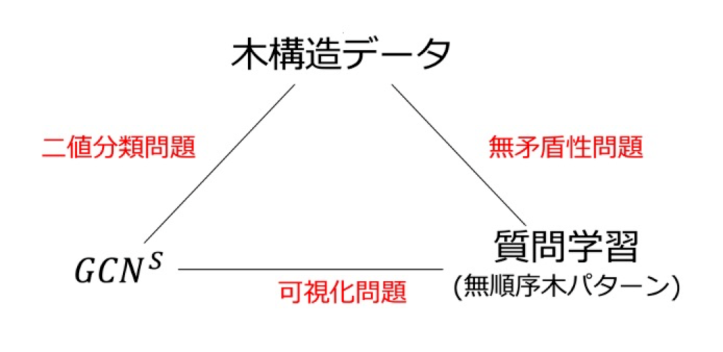
\includegraphics[scale=0.5]{fig-relation.eps}
  \caption{データとモデルの関係性: 木構造データ$S$は無順序木の正例集合$S_+$と負例集合$S_-$の和集合である.$S$を訓練データとした学習済みGCNを$GCN^S$と記す.}\label{fig:relation}
\end{figure}

協調モデルを効率的に解析するために,1つのサイズ$N$の正例を入力とするとき,所属性質問を$O(N)$回用いる新たな質問学習アルゴリズムを提案し,その性能を実験的に評価する.このアルゴリズムは,少数の質問回数で正確な結果を得ることを目的としており,従来の手法に比べて効果的である.また,ある特定のグラフ畳み込み層と組み合わせることで高い精度を達成する.さらに,今後の研究の方向性として,順序木における構造のバランス化を通じた効率化を検討する.具体的には,順序木のバランス化を行うことで,その高さを抑制し,構造の深さに依存する処理を軽減することを目指す.このアプローチにより,特に木構造間のマッチング判定において,高速な解析が可能となることが期待される.この手法は,本論文が提案する質問学習アルゴリズムのさらなる発展の基盤となる.

%\section*{本論文の構成}
%第2章では,本論文の基礎となる内容として,グラフの基本的な用語,線形無順序木パターン,および線形順序項木パターンの定義について述べる.
%第3章では,線形無順序木パターンに対する質問学習モデルと所属性質問について述べ,無順序木パターンの無矛盾性問題がNP完全であることを証明する.その後,一つの正例とそのサイズに比例した回数の所属性質問を用いる新たな質問学習アルゴリズムを提案し,その正当性を理論的および実験的に示す.
%第4章では,オラクルとしてGCNを用いる質問学習モデルを定義し,その性能を実験的に評価する.
%第5章では,バランス化推論システムについて述べる.
%第6章では,本論文の結果をまとめるとともに,本研究の今後の課題について述べる.